    \documentclass[conference]{IEEEtran}
    
    \usepackage{graphicx}
    \usepackage{biblatex}
    \usepackage{multicol}
    \usepackage[utf8]{inputenc}
    \usepackage{xepersian}
    
    \bibliographystyle{ieeetr-fa}
    \settextfont{Gandom.ttf}
    \addbibresource{bib.bib}
    \renewcommand{\thesection}{\arabic{section}}
    \usepackage{blindtext, graphicx}
    \hyphenation{op-tical net-works semi-conduc-tor}
    
    \usepackage{blindtext, graphicx}
    
    \title{دسته بندی اتوماتیک ژانر موسیقی   }
    \author{
    امیر حسین باقری\\
    مصطفی لسانی\\
    حسین کافی
    }
    \date{پاییز 97}
    \renewcommand\footnoterule{\kern-3\hrule\kern2.6}
    
     
    
    \begin{document}
    \maketitle
    
    
    
        \section{چکیده} 
این مقاله به بررسی راه حلی برای تولید پلی لیست های آهنگ به صورت اتوماتیک به کمک الگوریتم های یاد‌گیری ماشین پرداخته است. داده‌های استفاده شده در این پروژه از ۷ ژانر پاپ, کلاسیک, چیل, پانک, متال, تکنو و اکوستیک می‌باشد. تعداد کل آهنگ‌ها ۱۴۰ عدد و تعداد آهنگ‌های هر ژانر ۲۰ عدد می‌باشد. استخراج ویژگی از سیگنال آهنگ به کمک کتابخانه لیبروزا پایتون انجام شده است. از الگوریتم خوشه بندی کی میانگین برای ساخت پلی لیست آهنگ و خوشه بندی آهنگ‌ها استفاده شده است. کارایی این برنامه برای سه ژانر 16.78 درصد, برای پنج ژانر 4.58  درصد و برای ۷ ژانر 69.43  در صد بوده است.

    
    \section{مقدمه} 
    موسیقی تاثیر پر رنگی در زندگی روزمره انسان ها دارند. انسان ها برای کاهش استرس های درونی و برونی، از بین بردن خستگی، به دست آوردن آرامش و ... به موسیقی روی می آورند. طبق سایت آماری نلسون، مردم آمریکا روزانه چهار و نیم ساعت به آهنگ گوش می دهند. این نشان میدهند که خوب یا بد، نقش موسیقی در زندگی انسان ها بسیار پر رنگ است. 
ممکن است بار ها برای شما اتفاق افتاده باشد که بخواهید آهنگ گوش کنید ولی هر چه به آهنگ های گوشی موبایل یا لپتاپتان گوش میدهید خوشتان نمی آید یا به عبارتی با حس آن لحظه شما هماهنگ نیست. خیلی از ماها در این لحظات به دنبال یک پلی لیستی هستیم که آهنگ های مورد نظرمان در آن لیست باشد. مثلا صبح تازه رفتیم سر کار، و انرژی فراوانی داریم، دوست داریم به آهنگ های شاد گوش کنیم. غروب که از سر کار بر میگردیم به دلیل خستگی دوست داریم آهنگ آرام و غمگین گوش کنیم. راه حل این مشکل ساخت پلی لیست است، اما ساخت پلی لیست می تواند بسیار زمان بر و خسته کننده باشد.
در این پروژه هدف ما حل مشکلات ذکر شده در بالا است. ما پروسه ساخت پلی لیست را اتوماتیک کرده و آهنگ ها را با تکنیک ها و الگوریتم های یاد گیری ماشین طبقه بندی کردیم به طوری که آهنگ هایی که از نظر سیگنالی با هم شباهت دارند در یک دسته قرار بگیرند. در ادامه نمونه های مشابه این پروژه را بررسی میکنیم و تفاوت آن ها با این پروژه را توضیح میدهیم. 
    \section{کار های مشابه}
    شرکت ها و سازمان های زیادی در این زمینه سرمایه گذاری کردند. یکی از نمونه های بسیار پخته این برنامه توسط شرکت اسپاتیفای پیاده سازی شده است که به طور روزانه بر اساس آهنگ هایی که تا به حال گوش داده اید پلی لیست هایی را با عنوان daily mix تولید می کند.  شرکت های دیگری هم چون iTunes, amazon  نیز این سیستم را که تحت عنوان سیستم پیشنهاد دهنده \LTRfootnote{ Recommender system } شناخته می شود پیاده سازی کرده اند.
سیستم های پیشنهاد دهنده آهنگ که به طور گسترده وجود دارند بر دو اساس کار می کنند. فیلتر کردن مشارکتی \LTRfootnote{ Collaborative filtering }  و فیلتر کردن مبنی بر محتوا \LTRfootnote{ Content-based filtering }. در سیستم فیلتر کردن مشارکتی، سیستم در مورد کاربر اطلاعاتی همچون علایق و سلایق را استخراج می کند و با توجه به اینکه کاربر های مشابه به چه آهنگ هایی گوش می دهند این آهنگ ها را به کاربر پیشنهاد می دهد. در مکانیزم فیلتر مبنی بر محتوا ، با استفاده از اطلاعات مربوط به آهنگ ها همچون ژانر، سال ، خواننده و ... آهنگ های مشابه را پیدا کرده و به کاربران نشان می دهند. در هر دو مکانیزم اطلاعات زیادی نیاز است تا این سیستم به درستی کار کند. در حالت فیلتر مشارکتی به تعداد زیادی کاربر نیاز است که علایق آنها مشخص شده و در حالت فیلتر مبنی بر محتوا نیز اطلاعات زیادی هم چون ژانر آهنگ ، سالی که آهنگ انتشار یافت ، خواننده و ... نیاز است. کاری که ما در این پروژه انجام دادیم بررسی سیگنال خام آهنگ ها و استخراج ویژگی از آنهاست. در نهایت این ویژگی ها توسط الگوریتم های یادگیری ماشین طبقه بندی می شوند. در این حالت دیگر مشکل نبود اطلاعات اولیه وجود ندارد.
    \section{ استخراج ویژگی \LTRfootnote{ Feature extraction } }
استخراج ویژگی یکی از مهمترین و پر چالش ترین بخش های این پروژه می باشد. دقت در استخراج ویژگی تاثیر مستقیم بر روی نتیجه نهایی می گذارد. به طوری که گفته می شود اگر این بخش درست انجام نشود، نتیجه نهایی اشتباه خواهد بود. 
این مرحله در پردازش انواع سیگنال ها اجتناب ناپذیر می باشد. یک سیگنال در یک بازه زمانی حاوی داده های نامربوط بسیاری می باشد که به صورت مستقیم می توان از آنها برای طبقه بندی استفاده کرد. مشکل اصلی در این زمینه یافتن ویژگی های موثری است که به روند طبقه بندی سرعت و دقت بالاتری بخشند. زیرا ویژگی های ضعیف علاوه بر دشوار ساختن عملیات طبقه بندی ، موجب دریافت نتایج ضعیف می گردند. در این راستا در ادامه انواع ویژگی های سیگنال های صوتی به اجمال مورد بررسی قرار می گیرند. 

    \subsection{ ویژگی های طیفی  }
ویژگی های طیفی ویژگی هایی هستند که یک طیف را در بازه های زمانی کوچک قابل تمایز می سازند. این ویژگی ها به خصوص درباره طبقه بندی سیگنال های صوتی بسیار موثر می باشند. اگر چه ویژگی های متفاوتی در مسایل مختلف قابل بحث هستند ، اما در مورد موضوعاتی مانند تشخیص آوا ها و ابزار های موسیقی ویژگی های موقتی از جایگاه ویژه ای برخوردارند.
در استخراج ویژگی های طیفی فاز مربوط به طیف قابل حذف است و به این منجر به 50 در صد کاهش اطلاعات خواهد شد. همچنین ساختار مناسب طیف در اکثر مواقع قابل حذف می باشد. همچنین می توان بسیاری از اطلاعات نامربوط دیگر را حذف نمود. تنها چیزی که باقی می ماند طیف ضخیم مربوط به توزیع انرژی می باشد که در طبقه بندی سیگنال های صوتی از اهمیت بالایی بر خوردار می باشد و در واقع پایه ای برای تشخیص ویژگی های گفتار و آوا های صوتی می باشد.
    \subsubsection{ ضرایب Cepstral }
    ضرایب Cepstral که با c(k) نشان داده می شوند یک راه بسیار مناسب برای مدل کردن توزیع انرژی طیف می باشند.این ضرایب به صورت زیر قابل محاسبه اند
    \begin{equation}
        C (k) & = IDFT {\log |DFT{x(n)}|}
    \end{equation}
که DFT تبدیل فوریه و IDFT معکوس آن می باشد.
از آنجا که دقت عددی تولید شده بسیار کم اهمیت می باشد در فرمول بالا جز حقیقی به عنوان c در نظر گرفته شده است. ضرایب Cepstral در فریم های کوتاهی در طول زمان محاسبه می شوند که البته مدل های محاسبه شده با محاسبه میانگین و واریانس هر ضریب در طول زمان قابل افزایش است. فقط از M ضریب اول Cepstral به عنوان ویژگی استفاده می شود. در مورد این ضرایب نکات زیر حائز اهمیت است :
    \begin{itemize}
    \item  در صورت استفاده از کلیه ضرایب طیف به صورت دقیق به دست می آید.
    \item شمای طیف ضخیم با استفاده از ضرایب ابتدایی به دست می آید.
    \item دقت مدل سازی با توجه به تعداد ضرایب تعیین می شود.
    \item اولین ضریب که انرژی می باشد دور انداخته می شود.    
    \end{itemize}
مشکل عمده در استفاده از ضرایب Cepstral خطی بودن مقیاس فرکانس می باشد. زیرا معمولا فرکانس هایی که در محدوده 100 تا 200 هرتز و 10 تا 20 کیلو هرتز هستند دارای اهمیت می باشند که ضرایب Cepstral این محدوده را به حساب نمی آورند. در این شرایط به نظر می آید که مقیاس لگاریتمی از فرکانس بتواند عملکرد بهتری داشته باشد. برای حل این مشکل باید توجه داشت که عمدتا ما به دنبال تشابهات و عدم تشابهات در مورد ادراک ها برای طبقه بندی هستیم ضمن اینکه ویژگی های مرتبط استخراج شده از این ادراک ها ما را به سمت یک کلاس بندی مطلوب هدایت می کند. بنابراین در راستای رسیدن به هدف نیاز به مرغوب سازی ویژگی ها با اعمال اندکی تغییر در آنها احساس می شود. البته باید توجه داشت که اعمال تغییرات کوچک در ویژگی ها منجر به اعمال تغییرات کوچک در داده های ادراکی می شود(و بالعکس). به دلیل پایین بودن وضوح این تغییرات به خاطر مناسب نبودن مقیاس نیاز به ضرایبی با درجه وضوح بالاتری در نشان دادن این تغییرات جزیی داریم. این نیاز منجر به استفاده از ضرایب جدیدی تحت عنوان ضرایب Mel-frequency cepstral می شود که به طور کامل کمبود های یاد شده را پوشش می دهد.در ادامه به بررسی تاثیر انواع مقیاس ها بر روی کیفیت خواهیم پرداخت.
\subsubsection{ ضرایب Mel-Frequency-cepstral }
این ضرایب نوع بهبود یافته از ضریب cepstral می باشند. استفاده از ویژگی MFCCs  در سیستم‌های تشخیص صحبت  بسیار رایج است. از این ویژگی همچنین در استخراج اطلاعات از آهنگ  مانند طبقه بندی ژانر موسیقی نیز استفاده می‌شود.
مراحل کار برای تولید این ضرایب به این صورت است که پس از پنجره بندی و ایجاد فریم ها از سیگنال ورودی تبدیل فوریه گسسته بر روی هر یک از این فریم ها اعمال شده و حاصل به filterbank داده می شود. این فیلتر بر روی دامنه فرکانس ها اعمال شده و آن را یکنواخت می سازد. یک راه برای تولید Mel-frequency درونیابی بر روی فرکانس گسسته اصلی می باشد. پس از اعمال فیلتر و سپس تبدیل cosine گسسته(DCT) MFCC بدست آمده است.
مقیاس مورد استفاده در فرکانس Mel به صورت زیر محاسبه می شود :
\begin{equation}
    Mel(f)=2595 \log (1+\frac{f}{700})
\end{equation}
پس از محاسبه این ضریب در ادامه به پاره ای از دلایل موفقیت این ضریب خواهیم پرداخت. یکی از دلایل کارایی بالا این ضریب در درجه وضوح بالای آن می باشد. به این معنی که تغییرات جزیی با استفاده از این مقیاس اثر خود را به خوبی نشان می دهند. نقطه قوت دیگر این روش در استفاده از DCT می باشد که علاوه بر اینکه spectral fine structure را حذف می کند و باعث خلاصه سازی داده ها می شود همبستگی بین ویژگی ها را از بین برده و عملیات طبقه بندی را بهبود می بخشد.
MFCC   در کنار سایر ویژگی ها می تواند به صورت یک بردار پیوسته از ویژگی ها بیان شود. به عنوان یکی از ویژگی های مورد استفاده در کنار MFCC می توان به مرکز ثقل طیف اشاره کرد. ویژگی دیگر قابل بررسی درباره طیف پهنای باند آن می باشد. به عنوان ویژگی های دیگر به خصوص درباره صدا های موزون می توان به بی نظمی طیفی اشاره کرد که در واقع انحراف از دامنه های موزون طیف می باشد. 
    \begin{figure}[h!]
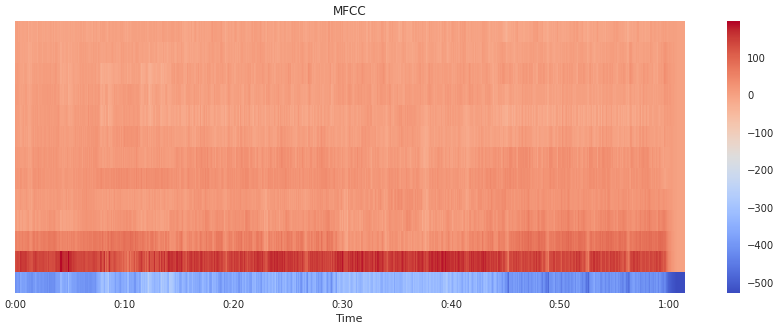
\includegraphics[width=\linewidth]{3.png}
      \caption{  ویژگی MFCCs }
      \label{fig:fig 1}
    \end{figure}
\subsubsection{ مرکز ثقل دامنه های طیفی \LTRfootnote{ Spectral Centroid }  }
طیف سنجی بر اساس مرکز مقیاسی است که در پردازش سیگنال دیجیتالی برای توصیف کردن طیف به کار می‌رود. این مقیاس مشخص می کند مرکز ثقل طیف در کجا قرار دارد. این ویژگی از طریق میانگین وزنی فرکانسی که درون سیگنال وجود دارد به دست می آید. وزن سیگنال از طریق اندازه تبدیل فوریه سیگنال در آن پنجره به دست می آید.
\begin{equation}
    Centroid = \frac{\sum_{n=1}^{N-1}f(n)x(n)}{\sum_{n=1}^{N-1}x(n)}
\end{equation}
در فرمول بالا x(n) وزن یا اندازه فرکانس را در یک پنجره نشان می دهد وf(n)  مرکز فرکانس را در پنجره مشخص میکند.
    \begin{figure}[h!]
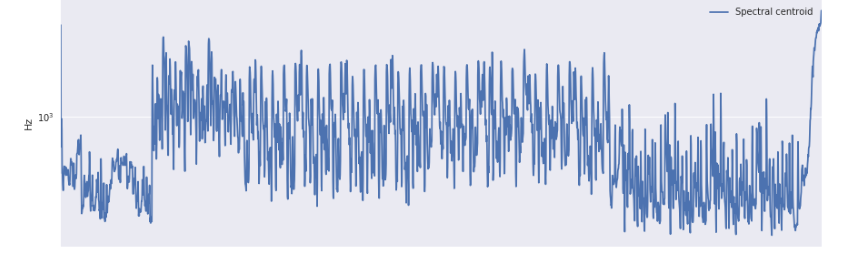
\includegraphics[width=\linewidth]{4.png}
      \caption{  مرکز ثقل دامنه های طیفی }
      \label{fig:fig 1}
    \end{figure}
    \subsubsection{ طیف سنجی بر اساس تضاد  \LTRfootnote{ Spectral Contrast }     }
طیف سنجی بر اساس تضاد نیز برای توصیف آهنگ توسعه یافت. این ویژگی، قله و دره را در هر زیر باند به طور جدا گانه در نظر میگیرد. به طور کلی، قله طیف نمایانگر جز هارمونیک و دره طیف نمایانگر بخش غیر هارمونیک یا نویز می‌باشد. بنابراین تفاوت میان قله طیف و دره طیف، بازتاب توزیع تضاد موجود در طیف است.
    \begin{figure}[h!]
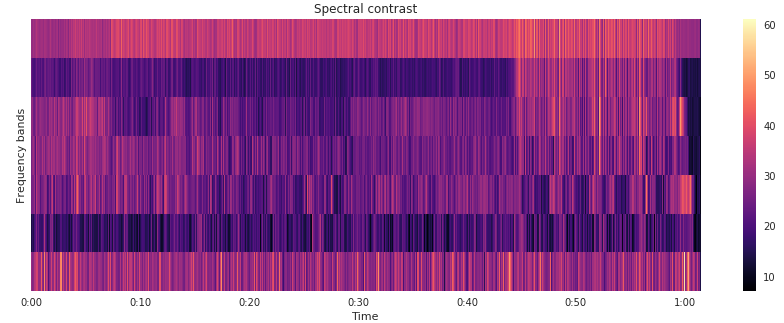
\includegraphics[width=\linewidth]{5.png}
      \caption{  طیف سنجی بر اساس تضاد }
      \label{fig:fig 1}
    \end{figure}
    \subsubsection{ نرخ عبور از صفر \LTRfootnote{ Zero crossing rate }     }
نقطه عبور از صفر نقطه‌ای است که دامنه سیگنال در در آن نقطه صفر است. در نقاط دیگر، دامنه  موج یا به سمت قله می‌رود یا به سمت دره نزول میکند .نرخ عبور از صفر، نرخی است که مقدار سیگنال در آن از مثبت به منفی تبدیل می شود یا بر عکس. این ویژگی به طور مکرر در تشخیص صدا و استخراج اطلاعات از آهنگ به کار می رود. 
رابطه ریز برای محاسبه نرخ عبور از صفر به کار می رود.
\begin{equation}
    zcr=\frac{1}{T-1}\sum_{t=1}^{T-1}I_{R<0} (S_t S_{t-1})
\end{equation}
که در این فرمول S سیگنال به طول T می باشد و I_(R<0) که تابع همانی می باشد. گاهی اوقات ما فقط تعداد مثبت شدن یا فقط تعداد منفی شدن را محاسبه می کنیم، به جای اینکه همه حالت ها را محاسبه کنیم. زیرا همواره تعداد مثبت شدن یا منفی شدن یا با هم برابر است یا یک عدد کمتر یا بیشتر است که برای ما اهمیتی ندارد.
    \subsection{ ویژگی نت محتوا  \LTRfootnote{ Pitch content features }     }
ویژگی نت محتوا به نت های مربوط به آهنگ مربوط می شود که در نتیجه این ارتباط، به ملودی آهنگ نیز ارتباط پیدا می کند. نحوه پیدا کردن نت ها درون آهنگ به طور کلی به این صورت است که هر نوت یک دامنه فرکانس خاص و انرژی خاصی دارد. این فرکانس به ما کمک می کند تا بتوانیم نت های آهنگ را پیدا کنیم. در شکل زیر نمونه ای از این ویژگی را می بینید که تعداد هر یک از نت ها را در یک آهنگ به صورت نمودار نشان داده است.
\begin{figure}[h!]
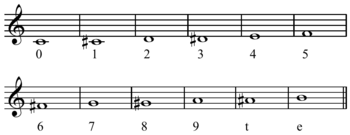
\includegraphics[width=\linewidth]{7.png}
      \caption{ نت های موسیقی }
      \label{fig:fig 1}
    \end{figure}

\begin{figure}[h!]
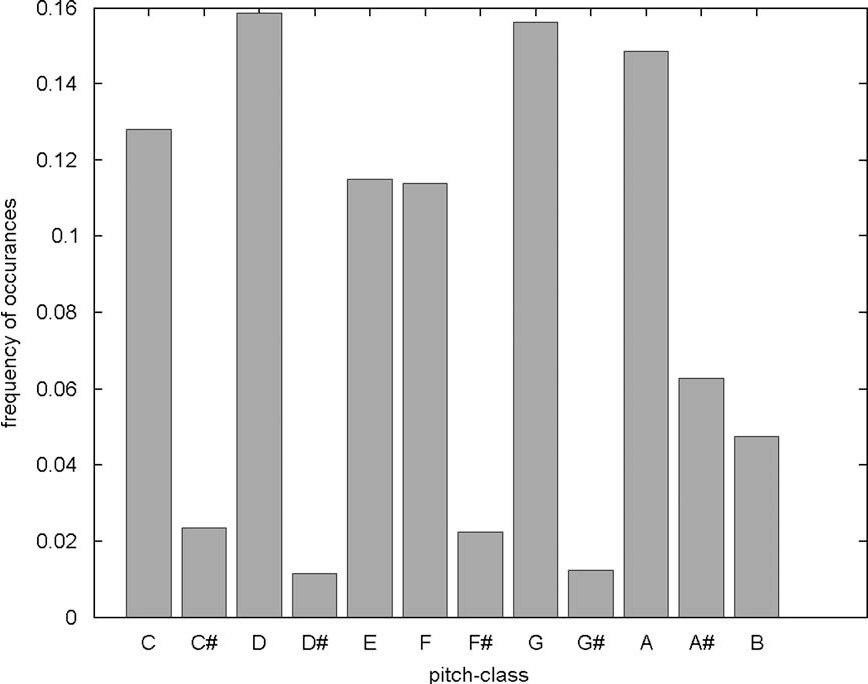
\includegraphics[width=\linewidth]{8.jpg}
      \caption{ نمونه ای از ویژگی استخراج شده از نت محتوا }
      \label{fig:fig 1}
    \end{figure}


    \subsubsection{ ویژگی CENS \LTRfootnote{ Chroma Energy Normalized }     }
    در موسیقی ویژگی کروما ارتباط بسیار نزدیکی با 12 نت موسیقی (7 نت اصلی و 5 نت نیم پرده) دارد. استخراج ویژگی بر اساس کروما ابزار بسیار قدرتمندی را برای طبقه بندی بر اساس نت موسقی به ما می‌دهد. ویژگی اصلی کروما این است که ویژگی ملودیک و هارمونیک آهنگ را استخراج کند.
این ویژگی ها بسیار قدرتمند هستند و ارتباط بسیار مستقیمی را با هارمونی آهنگ نشان می دهند. این دلیلی است که همراه این ویژگی در فرایند آنالیز داده های آهنگی استفاده می شود. برای مثال می توان گفت تقریبا برای همه برنامه های تشخیص صدا از این ویژگی یا شاخه ای از این ویژگی استفاده می شود. از دیگر کاربرد های این ویژگی میتوان به تشخیص آهنگ اشاره کرد که در برنامه های معروف شازم \LTRfootnote{ Shazam }      و موزیکسمچ \LTRfootnote{ Musixmatch }    اشاره کرد.
\begin{figure}[h!]
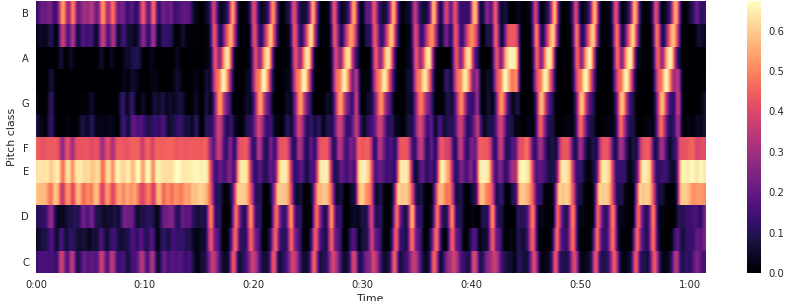
\includegraphics[width=\linewidth]{1.png}
      \caption{ Chroma Energy Normalized }
      \label{fig:fig 1}
    \end{figure}
    \subsection{ ویژگی ریتمی \LTRfootnote{ Rhythmic Feature }  }
    \subsubsection{ بیت \LTRfootnote{ Beat }  آهنگ }
کلمه بیت در لغت به معنای ضربان و یا ضرب در موسیقی می باشد که استفاده از آن در بین تنظیم کنندگان بسیار مرسوم است. بیت در موسیقی واژه‌ای است که قالبا به ریتم یک آهنگ گفته می‌شود. میانگین فاصله زمانی بین دو بیت به عنوان ویژگی ریتمی از آهنگ شناخته می شود.
\begin{figure}[h!]
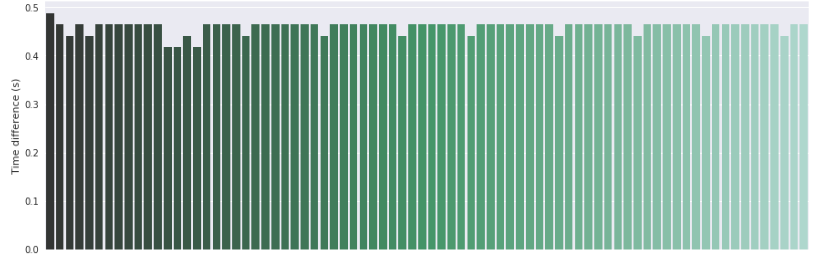
\includegraphics[width=\linewidth]{9.png}
      \caption{  نمونه ای از ریتم استخراج شده از آهنگ }
      \label{fig:fig 1}
    \end{figure}
        \subsection{ چالش ها و مشکلات استخراج ویژگی } 
در این بخش در مورد استخراج ویژگی از سیگنال آهنگ بحث کردیم. اما این شکل استخراج ویژگی با مشکلات فنی همراه است. مشکلات به در نظر نگرفتن ویژگی ذاتی ژانر موسیقی می باشد. در دنیای موسیقی، ژانر موسیقی به وسیله سازندگان اثر یا افراد موسیقی دان طبقه بندی می شود. ژانر ها بر اساس یک سری قرار داد که بین موسیقی دانان وجود دارند تعیین می شوند. گاها این ویژگی ها می تواند به ویژگی های فرهنگی و ملی یک گروه یا کشور نیز مربوط شود. حتی متن موسیقی هم می تواند روی ژانر موسیقی تاثیر بگذارد. نکته دیگر این است که یک آهنگ ممکن است چند ژانر مختلف را هم زمان داشته باشد، اما ما برای ساده سازی پیاده سازی فرض کردیم که یک آهنگ فقط می تواند یک ژانر داشته باشد. همچنین هیچ متن کاوی \LTRfootnote{ Text-mining }    روی متن موسیقی \LTRfootnote{ Lyrics }   انجام نداده ایم. 
انجام این بهینه سازی ها میتواند دقت خوشه بندی را بسیار بالا ببرد. اما با توجه به اینکه پیاده سازی موارد گفته شده کار بسیار حرفه ای و دشوار است و به افراد متخصص از رشته های مختلف ، هم چون موسیقی ،پردازش سیگنال، تئوری موسیقی، متن کاوی و ... نیازمند است.

        \section{ الگوریتم } 
برای ساخت پلی لیست راه های گوناگونی وجود دارد، یکی از این راه ها طبقه بندی بر اساس ژانر موسیقی می باشد. طبقه بندی بر اساس ژانر نیازمند داده است که از قبل طبقه بندی شده اند و با استفاده از الگوریتم های طبقه بندی \LTRfootnote{ Classification }  به صورت نظارت شده \LTRfootnote{ Supervised }  داده ها را طبقه بندی کنیم. راه حل دیگر نیز برای طبقه بندی داده ها وجود دارد که به آن طبقه بندی نظارت نشده \LTRfootnote{ Unsupervised }   گفته می شود. در روش نظارت نشده نیازی به داده طبقه بندی شده نیست. طبقه بندی نظارت نشده، داده ها را بر اساس شباهتشان در یک دسته قرار می دهد. از آنجایی که در حالت نظارت نشده نیازی به داده اضافی نیست ما از این راه حل استفاده کردیم. در ادامه توضیحات کامل تری درباره طبقه بندی نظارت شده و نشده ارائه خواهد شد.
        \subsection{ یادگیری نظارت شده } 
یادگیری با نظارت یا یادگیری تحت نظارت یکی از زیرمجموعه‌های یادگیری ماشینی است. با یک مثال عمومی وارد این بحث می‌شویم. یک میوه فروشی را در نظر بگیرید که تمام میوه ها را بصورت کاملاً جدا از هم مرتب کرده‌است و شما نوع میوه را کاملاً می دانید، یعنی زمانی که یک میوه را در دست می گیرید به نام نوشته شده در قفسه آن نگاه می کنید و در میابید که مثلاً سیب است و اصطلاحاً می گویند تمام داده ها تگ گذاری شده هستند. به طبع فردی از قبل دسته داده‌ها را مشخص کرده‌است. حال اگر با دید موجودی در حال یادگیری به ماجرا نگاه کنیم، انتظار می‌رود فرضاً مفهومی از سیب‌ها را یاد بگیرد و احتمالاً در آینده نیز اگر تصویری از سیب‌ها دید آن را تشخیص دهد.
این روش ، یک روش عمومی در یادگیری ماشین است که در آن به یک سیستم، مجموعه ای از جفت‌های ورودی – خروجی ارائه شده و سیستم تلاش می‌کند تا تابعی از ورودی به خروجی را فرا گیرد. یادگیری تحت نظارت نیازمند تعدادی داده ورودی به منظور آموزش سیستم است. با این حال رده‌ای از مسائل وجود دارند که خروجی مناسب که یک سیستم یادگیری تحت نظارت نیازمند آن است، برای آن‌ها موجود نیست. این نوع از مسائل چندان قابل جوابگویی با استفاده از یادگیری تحت نظارت نیستند. یادگیری تقویتی \LTRfootnote{ Reinforced learning }  مدلی برای مسائلی از این قبیل فراهم می‌آورد. در یادگیری تقویتی، سیستم تلاش می‌کند تا تقابلات خود با یک محیط پویا را از طریق آزمون و خطا بهینه نماید. یادگیری تقویتی مسئله‌ای است که یک عامل که می‌بایست رفتار خود را از طریق تعاملات آزمون و خطا با یک محیط پویا فرا گیرد، با آن مواجه است. در یادگیری تقویتی هیچ نوع زوج ورودی- خروجی ارائه نمی‌شود. به جای آن، پس از اتخاذ یک عمل، حالت بعدی و پاداش بلافصل به عامل ارائه می‌شود. هدف اولیه برنامه‌ریزی عامل‌ها با استفاده از تنبیه و تشویق است بدون آنکه ذکری از چگونگی انجام وظیفه آن‌ها شود.
یک مجموعه از مثالهای یادگیری وجود دارد بازای هر ورودی، مقدار خروجی یا تابع مربوطه نیز مشخص است. هدف سیستم یادگیر بدست آوردن فرضیه‌ای است که تابع یا رابطه بین ورودی یا خروجی را حدس بزند به این روش یادگیری با نظارت گفته می‌شود. مثالهای زیادی در یادگیری ماشینی وجود دارند که در دسته یادگیری با نظارت میگنجند، از جمله می‌توان به درخت تصمیم‌گیری \LTRfootnote{ Decision tree }، آدابوست \LTRfootnote{ AdaBoost }، ماشین بردار پشتیبانی \LTRfootnote{ Support Vector Machine }، دسته‌بندی‌کننده بیز ساده\LTRfootnote{ Naive Bayes classifier }، رگرسیون خطی \LTRfootnote{ Linear regression }، رگرسیون لجستیک\LTRfootnote{ Logistic regression }، شبکه‌های عصبی\LTRfootnote{ Artificial Neural Networks - ANN } و بسیاری مثالهای دیگر اشاره کرد.
از آنجایی که در این پروژه از این روش یادگیری استفاده نشده است به همین توضیحات اکتفا کرده و وارد توضیح الگوریتم های این روش نمی شویم.

        \subsection{ یادگیری نظارت نشده و خوشه بندی \LTRfootnote{ Clustering }  } 
این مدل ماشین بدون استفاده از داده های برچسب گذاری شده و بدون هیچ معلمی می آموزد. به حالت ساده تر می توان گفت که در ابتدا تمامی نمونه هایی که به آن داده می شوند، هیچ برچسبی ندارند در صورتی که در یادگیری نظارتی تمامی داده ها برچسب داشتند. به عنوان مثال، ایمیل های اسپم و غیر اسپم. در یادگیری بدون نظارت برچسبی بر روی داده ها وجود ندارد.
الگوریتم های مصور سازی  مثالی است که برای یادگیری بدون نظارت می توان زد. به عنوان مثال شما تعداد بسیار زیادی به آن عکس می دهید و هیچ برچسبی هم بر روی عکس ها نمی گذارید. (مثلا عکس ماشین به آن می دهید و نمی گویید که این ماشین است). الگوریتم مورد نظر تلاش می کند تا ساختاری میان آن ها پیدا کند و آن ها را خوشه بندی کند. درنهایت متوجه می شوند که چطور داده را سازماندهی کنند.
خوشه‌بندي یکی از مهمترین ابزار کشف داده‌ها است که در کشف هاي تصادفی به کار گرفته می‌شود. در حال حاضر، اخذ دانش یک گلوگاه عمده در فرآیند مهندسی دانش محسوب می‌شود. الگوریتم‌هاي یادگیري ماشین و داده‌کاوي با هدف استخراج دانش از داده‌ها، به عنوان روشی براي حل این مشکل مطرح می‌باشند. یک رهیافت متداول در این زمینه روش خوشه‌بندي است که براي تصمیم‌گیري یا دسته‌بندي یا کلاس‌بندي می‌تواند تصمیمات نمادینی را به نمونه‌هاي جدید با استفاده از نمونه‌هاي موجود منتسب کنند. روش‌هاي خوشه‌بندي به واسطه قابلیت درکی که در خود نهفته دارند، از اقبال خوبی برخوردار شده‌اند. وجود قابلیت درك از جهات گوناگونی حائز اهمیت می باشد. فهم قلمرو، درك قابلیت‌هاي کلاس‌بندي، توجیه تصمیم و بالاخره وجود قوانین نمادینی که می‌توانند از روي خوشه‌هاي استخراج شده و سپس در یک سیستم تصمیم‌گیري مبنی بر قوانین به کار گرفته شوند.
خوشه‌بندي در واقع یک عملیات غیر‌نظارتی می باشد. این عملیات هنگامی استفاده می‌شود که ما به دنبال یافتن گروه‌هایی از داده‌هاي مشابه می‌باشیم بدون این‌که از قبل پیش‌بینی در مورد شباهت‌هاي موجود داشته باشیم. خوشه‌بندي معمولاً هنگامی استفاده می‌شود که به دنبال یافتن گروه‌هایی از مشتریان هستیم که قبلا شناخته نشده‌اند. براي مثال می‌توان شباهت‌هاي مشتریان در استفاده از تلفن‌همراه را به منظور گروه‌بندي مشتریان و تشخیص خدمت جدیدي جستجو نمود.
از الگوریتم های مربوط به یادگیری نظارت نشده می توان الگوریتم کی-میانگین\LTRfootnote{ K-mean }   و DBSCAN را نام برد. در ادامه در مورد این الگوریتم ها توضیح مختصری می بینید. 

        \subsubsection{ الگوریتم DBSCAN  } 
DBSCAN یک روش خوشه‌بندی  است که توسط مارتین اِستر، هانس-پتر کریگل، یورگ ساندر و شیائووی شو در ۱۹۹۶ میلادی (۱۳۷۵ شمسی) ارائه گردیده‌است. مزیت این روش به نسبت روش‌های دیگری خوشه‌بندی مانند خوشه‌بندی کی-میانگین این است که نسبت به شکل داده‌ها حساس نمی‌باشد و می‌تواند اشکال غیر منظم را نیز در داده‌ها تشخیص دهد.
 در شکل زیر نقاط قرمز رنگ نقاط مرکزی هستند. نقاط زرد به خوشه مشخص شده دسترسی دارند. نقطه آبی، نویز  است.

\begin{figure}[h!]
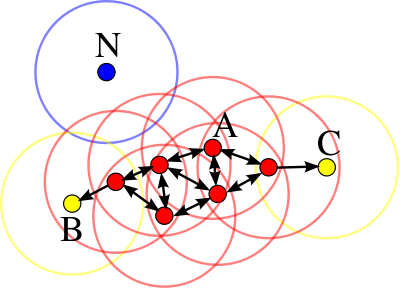
\includegraphics[width=\linewidth]{10.png}
      \caption{ انواع نقطه در DBSCAN  }
      \label{fig:fig 1}
    \end{figure}
        \subsubsection{ الگوریتم کی میانگین } 
خوشه‌بندی کی-میانگین روشی در کمی‌سازی بردارهاست که در اصل از پردازش سیگنال گرفته شده و برای آنالیز خوشه بندی در داده کاوی محبوب است. کی-میانگین خوشه‌بندی با هدف تجزیه n مشاهدات به k خوشه است که در آن هر یک از مشاهدات متعلق به خوشه ای با نزدیکترین میانگین آن است، این میانگین به عنوان پیش‌نمونه استفاده می‌شود. این به پارتیشن‌بندی داده‌های به یک دیاگرام ورونوی \LTRfootnote{ Voronoi diagram  }   تبدیل می‌شود.
اصطلاح کی-میانگین برای اولین بار توسط جیمز مک‌کوین در سال ۱۹۶۷ مورد استفاده قرار گرفت، هرچند این ایده به هوگو استینگز در سال ۱۹۵۷ باز می گردد. این الگوریتم ابتدا توسط استوارت لویید در سال ۱۹۵۷ به عنوان یک تکنیک برای مدولاسیون کد پالس پیشنهاد شد و تا سال ۱۹۸۲ خارج از آزمایشگاه‌های بل به انتشار نرسید. فورجی در سال ۱۹۶۵ الگوریتمی مشابه را منتشر کرد، به همین دلیل است که بعضی اوقات این الگوریتم، لویید فورجی هم نامیده می‌شود

\section{نتایج}
همانطور که در بخش داده ها گفته شده تعداد آهنگ ها 140 عدد و تعداد ژانر ها 7 عدد می باشد.در این پروژه داده ها را به سه دسته تقسیم کردیم. 
\begin{itemize}
    \item دسته اول: انتخاب 3 ژانر به تعداد 60 آهنگ 
    \item دسته دوم: انتخاب 5 ژانر به تعداد 100 آهنگ
    \item دسته سوم: انتخاب 7 ژانر به تعداد 140 آهنگ
\end{itemize}



این سه دسته خوشه بندی شده و نتایج آن در جدول 1 قابل مشاهده است .
\begin{table}[]
        \centering
    \begin{tabular}{|l|l|l|l|}
    \hline
    کارآیی & تعداد آهنگ  & تعداد ژانر  \\ \hline
    16.78 & 60 & 3 \\ \hline
4.58 & 100 & 5 \\ \hline
69.43 & 140 & 7 \\ \hline
    \end{tabular}
    \caption{نتایج خوشه بندی}
    \label{tab:my_label}
\end{table}


\begin{thebibliography}{99}
\begin{LTRbibitems}

\bibitem{1}
Soltau, H., Schultz, T., Westphal, M., Waibel, A. (1998).
Recognition of music types. In Acoustics, Speech and
Signal Processing, 1998. Proceedings of the 1998 IEEE
International Conference on (Vol. 2, pp. 1137-1140).
IEEE.

\bibitem{2}
Shao, X., Xu, C., Kankanhalli, M. S. (2004). Unsupervised
classification of music genre using hidden markov model.
In Multimedia and Expo, 2004. ICME’04. 2004 IEEE
International Conference on (Vol. 3, pp. 2023-2026).
IEEE.

\bibitem{3}
Cilibrasi, R., Vitányi, P., De Wolf, R. (2004). Algorith-
mic clustering of music based on string compression. In
Computer Music Journal on (Vol.28, no. 4, pp. 49-67).
IEEE.
\bibitem{4}
Tsai, W.H., Bao, D.F. (2010). Clustering music recordings
based on genres. In Information Science and Applications
(ICISA), 2010 International Conference on (pp. 1-5).
IEEE.
\bibitem{5}
Peng, W., Li, T., Ogihara, M. (2007). Music Clustering
with Constraints. In ISMIR (pp. 27-32).


\end{LTRbibitems}
\end{thebibliography}
 
    
    \end{document}

